Ne interesează să găsim \textit{cea mai bună strategie}. Pentru a compara între ele mai multe strategii, trebuie să gândim \textit{un mediu în care acestea să concureze}. 
 
Până la a găsi cea mai bună strategie, trebuie, mai întâi, să vedem cum anume poate configurația unui algoritm genetic să influențeze calitatea soluției. De asemenea, vrem să vedem cum anume se comportă într-un mediu de test strategia propusă de algoritm. 
 
Pentru a îndeplini aceste cerințe, am ales să supun cromozomii la un anumit tip de turneu, ce poartă denumirea de \textbf{turneu cu eliminare}.  

\section {Termeni întâlniţi}
O \textbf{rundă} este dată de alegerea, în mod secret, a mișcării următoare și actualizarea scorului în funcție de ce a pus și oponentul. 

Un \textbf{meci} este jucat de către doi jucători. Este alcătuit dintr-un număr de runde. În fiecare rundă, fiecare jucător alege, în mod secret, ce mișcare va face. La final de rundă, scorul jucătorilor este actualizat cu o valoare dată de mișcarea făcută de fiecare, în funcție de ce a ales și oponentul să facă. 

\section {Cum este modelat un turneu cu eliminare}
 
Un turneu cu eliminare pornește de la o populație de strategii în care, la fiecare iterație, fiecare individ joacă câte un meci cu ceilalți indivizi. Pe parcursul meciurilor, câștigurile individuale se însumează într-un scor total. După ce se joacă toate combinările de doi jucători (se ajunge la finalul iterației), se elimină un procent din cei mai slabi jucători.  Pentru a mai reduce din numărul parametrilor ale căror valori pot varia, am stabilit ca procentul să fie de 25\%. În caz de egalitate a scorurilor între doi jucători, se elimină la întâmplare unul din cei doi. Se completează locurile eliberate cu stategii care au obținut printre cele mai bune scoruri. Se resetează scorul total al indivizilor și se repetă acești pași până când în turneu a rămas un singur tip de strategie, ori până când am atins un număr maxim de iterații.  
\\\\
Observație: \textit{Când într-un turneu cu eliminare concurează doi indivizi ce au aceeași strategie deterministă, la finalul unei iterații, cei doi indivizi vor avea exact același scor. Nu putem spune același lucru despre doi indivizi care folosesc strategia \textbf{Random}.}
\\\\
Pentru a vedea clar modul în care evoluează strategiile în contextul acestui tip de turneu, am implementat o metodă grafică de vizualizare a datelor. Am ales să folosesc \textbf{line chart}-uri. Axa absciselor are drept legendă numărul de indivizi din fiecare strategie. Axa ordonatelor reprezintă numărul meciului din turneu.

\section{Configurația unui turneu cu eliminare}

Așa cum am stabilit parametrii mediului de antrenare (parametrii algoritmului genetic), va trebui să stabilim și în ce condiții vom testa cromozomii obținuți. Vom impune condiții legate de procentul de jucători care sunt eliminați, respectiv duplicați la final de iterație. De asemenea, vom stabili configurația populației de testare și câte copii după o anumită strategie a algoritmului genetic vor participa la turneul eliminatoriu. În ultimă instanță, vom alege numărul de runde ce va alcătui un meci dintre doi jucători. 
 
Cum s-a discutat în capitolul anterior, populația de testare va putea fi definită în fișierul \textbf{testing.config.json}.

În experimentele descrise, am ales ca participanții la turneu să aibă ponderi egale iar procentul de  jucători eliminați să fie de 25\%. 

\section {Concluzii trase în urma finalizării turneelor}

Fiecare experiment este dat de stabilirea parametrilor configurației algoritmului genetic, urmată de rularea algoritmului genetic și trecerea soluției prin mai multe medii de testare, prin varierea configurației turneului cu eliminare.

În contextul acestei probleme, nu putem vorbi despre optim local sau global, întrucât un fitness cu o valoare bună obținut pentru un cromozom în faza de antrenare poate să își piardă relevanța în faza de testare, datorită faptului că mediul de testare poate varia. 

În rândurile următoare prezint o serie de experimente.  

\subsection {Explorarea redusă a spațiului de căutare} 

\begin{center}
	\underline{\textit{Experimentul 1}}
\end{center}

\textit{Configurația algoritmului genetic și cea a turneului cu eliminare este trecută în \textbf{Anexa numărul 1}}.\\

Am făcut un prim experiment în care configurația algoritmului genetic a dus la o explorare redusă a spațiului de căutare. Pentru aceasta, am ales valori mici pentru numărul de generații (100), pentru numărul de runde din turneul clasic (10) și pentru probabilitățile operatorilor genetici (10\%).
 
Diagramele de mai jos atestă calitatea redusă a soluției obținute în urma rulării algoritmului genetic. 

\begin{figure}[H]
	\centering
	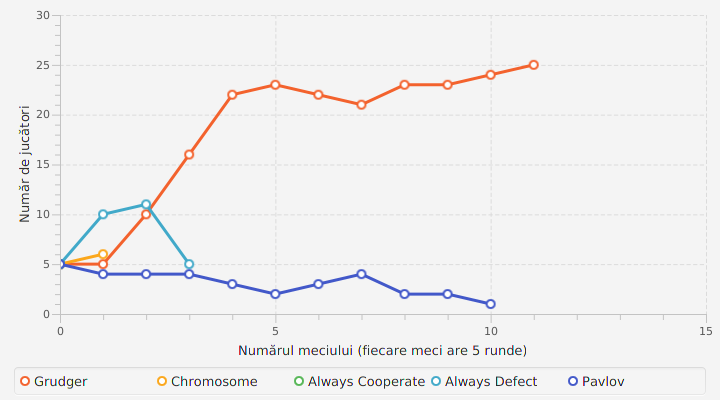
\includegraphics[	
	width=16cm,
	height=7.5cm,
	keepaspectratio
	]{imagini/experiment_1_epoch_1529303072346/chart_from_epoch_1529303304972.png}
	\caption{\textit{Cromozomii pierd în turneul cu eliminare cu 5 runde/meci.}}
\end{figure}

\begin{figure}[H]
	\centering
	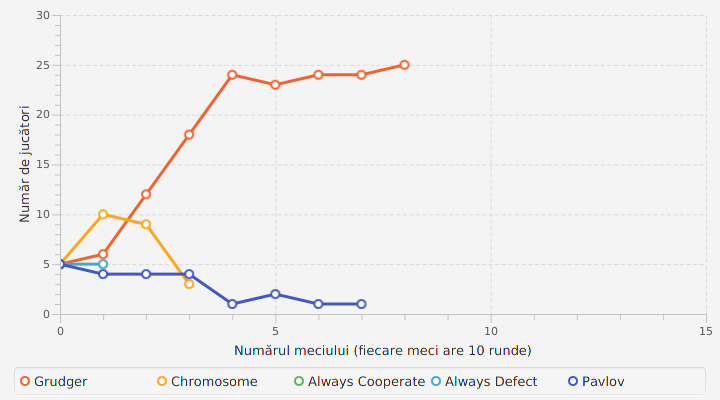
\includegraphics[	
	width=16cm,
	height=7.5cm,
	keepaspectratio
	]{imagini/experiment_1_epoch_1529303072346/chart_from_epoch_1529303340019.png}
	\caption{\textit{Cromozomii pierd în turneul cu eliminare cu 10 runde/meci.}}
\end{figure}

\begin{figure}[H]
	\centering
	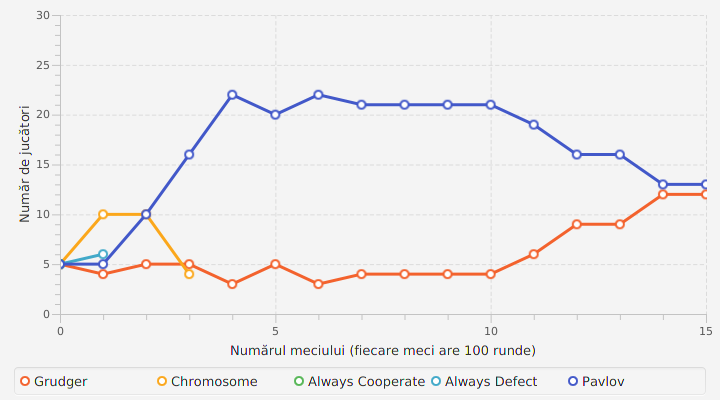
\includegraphics[	
	width=16cm,
	height=7.5cm,
	keepaspectratio
	]{imagini/experiment_1_epoch_1529303072346/chart_from_epoch_1529303352244.png}
	\caption{\textit{Cromozomii pierd în turneul cu eliminare cu 100 runde/meci.}}
\end{figure}

\begin{figure}[H]
	\centering
	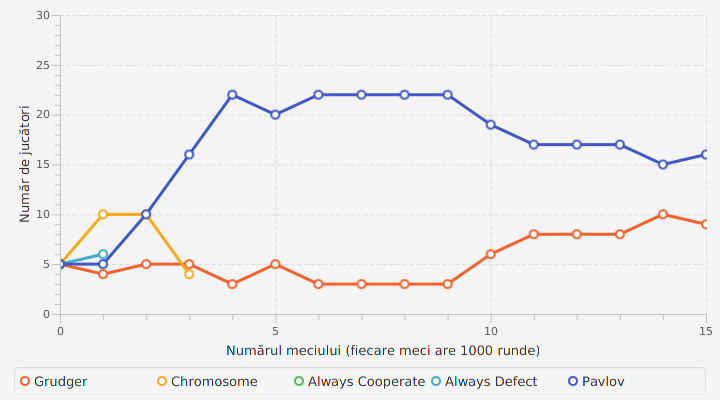
\includegraphics[	
	width=16cm,
	height=7.5cm,
	keepaspectratio
	]{imagini/experiment_1_epoch_1529303072346/chart_from_epoch_1529303371162.png}
	\caption{\textit{Cromozomii pierd în turneul cu eliminare cu 1000 runde/meci.}}
\end{figure}

\subsection {Numărul de runde al meciurilor din turneul cu eliminare}

\begin{center}
	\underline{\textit{Experimentul 2}}
\end{center}

\textit{Configurația algoritmului genetic și cea a turneului cu eliminare este trecută în \textbf{Anexa numărul 2}}.\\

Într-un alt experiment, am surpins cum numărul de runde al meciurilor din turneul cu eliminare, odată modificat cu o valoare foarte mică, a avantajat una din strategiile algoritmului genetic. 

\begin{figure}[H]
	\centering
	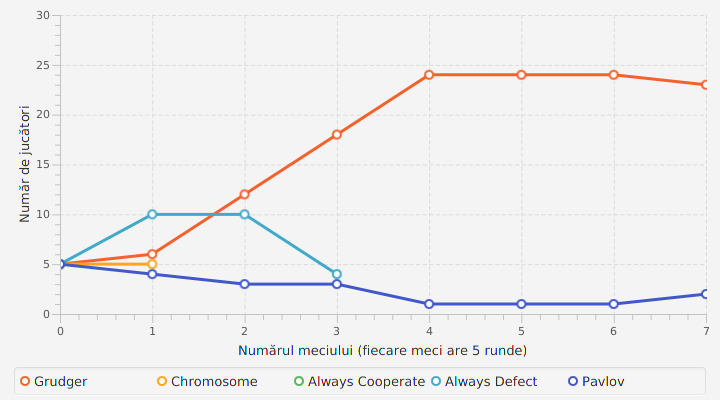
\includegraphics[	
	width=16cm,
	height=7.5cm,
	keepaspectratio
	]{imagini/experiment_2_epoch_1529309949939/chart_from_epoch_1529310422567.png}
	\caption{\textit{Cromozomii pierd în turneul cu eliminare cu 5 runde/meci.}}
\end{figure}

\begin{figure}[H]
	\centering
	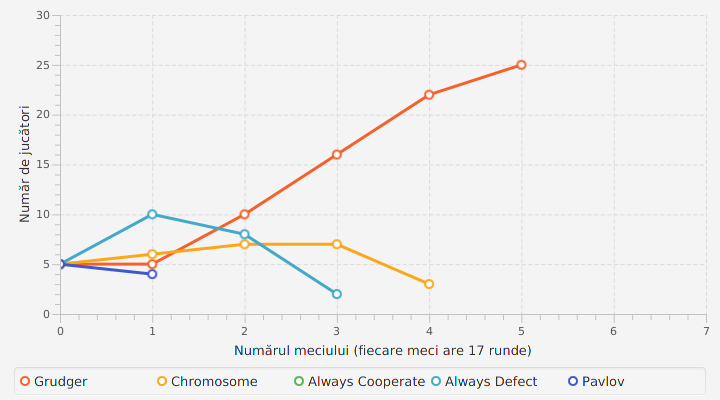
\includegraphics[	
		width=16cm,
		height=7.5cm,
		keepaspectratio
	]{imagini/experiment_2_epoch_1529309949939/chart_from_epoch_1529310399495.png}
	\caption{\textit{Cromozomii pierd în turneul cu eliminare cu 17 runde/meci.}}
\end{figure}

Mărind cu 1 numărul de runde din fiecare meci, observăm că strategia propusă de algoritmul genetic câștigă. 

\begin{figure}[H]
	\centering
	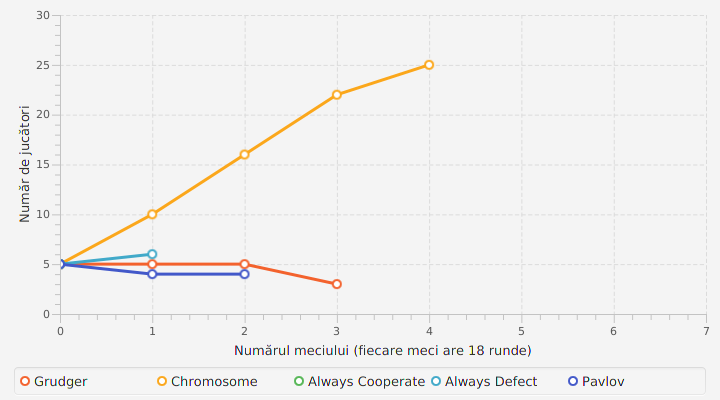
\includegraphics[	
	width=16cm,
	height=7.5cm,
	keepaspectratio
	]{imagini/experiment_2_epoch_1529309949939/chart_from_epoch_1529310386663.png}
	\caption{\textit{Cromozomii câștigă în turneul cu eliminare cu 18 runde/meci.}}
\end{figure}

\subsection{Strategia \textbf{Random}}

Strategia \textbf{Random} nu reprezintă o problemă pentru strategiile oferite de algoritmul genetic.

Am antrenat o populație de dimensiune mică (5 cromozomi) într-un număr mare de generații (1000), lansând valori mari ale mutației și încrucișării (50\% pentru ambii operatori). Populația de antrenament este dată de un singur individ de tip \textbf{Random}. Am rulat două experimente, în urma cărora am obținut două strategii: pentru prima strategie obținută, cea din experimentul numărul 3, numărul de runde al meciurilor tuneului clasic este mai mic (5 runde); pentru celălalt experiment numărul de runde al meciurilor din turneului clasic este 100.

\begin{center}
	\underline{\textit{Experimentul 3}}
\end{center}

\textit{Configurația algoritmului genetic și cea a turneului cu eliminare este trecută în \textbf{Anexa numărul 3}}.\\

\begin{figure}[H]
	\centering
	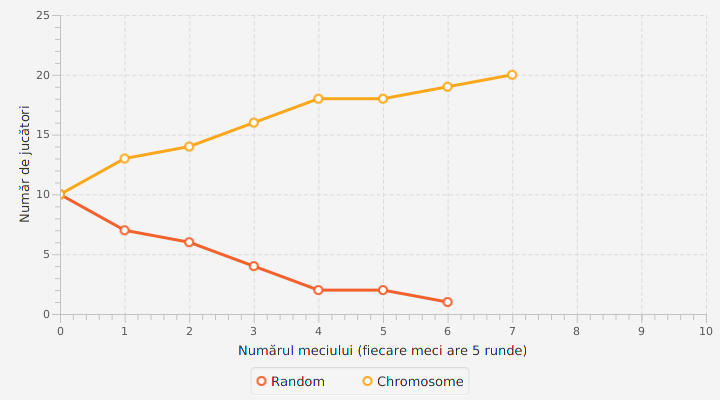
\includegraphics[	
	width=16cm,
	height=7.5cm,
	keepaspectratio
	]{imagini/experiment_3_epoch_1529321586156/chart_from_epoch_1529323404815.png}
	\caption{\textit{Cromozomii câștigă în turneul cu eliminare cu 5 runde/meci.}}
\end{figure}

\begin{figure}[H]
	\centering
	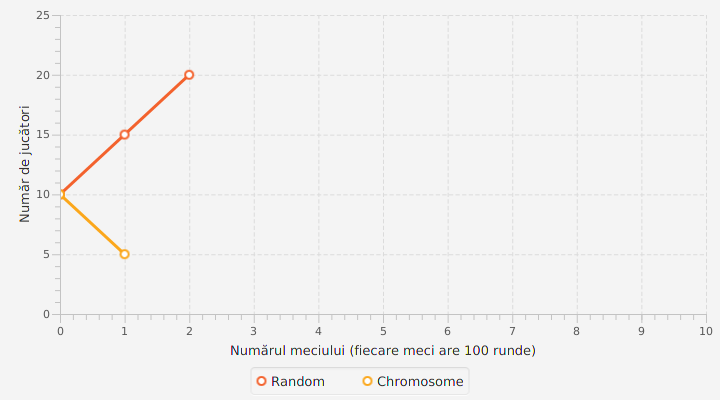
\includegraphics[	
	width=16cm,
	height=7.5cm,
	keepaspectratio
	]{imagini/experiment_3_epoch_1529321586156/chart_from_epoch_1529323424012.png}
	\caption{\textit{Strategia propusă de algoritmul genetic pierde, întrucât nu este optimizată pentru a câștiga în contextul unui turneu cu număr mare de runde.}}
	\label{pierde_cromozomul_castiga_random}
\end{figure}

\begin{center}
	\underline{\textit{Experimentul 4}}
\end{center}

\textit{Configurația algoritmului genetic și cea a turneului cu eliminare este trecută în \textbf{Anexa numărul 4}}.\\

\begin{figure}[H]
	\centering
	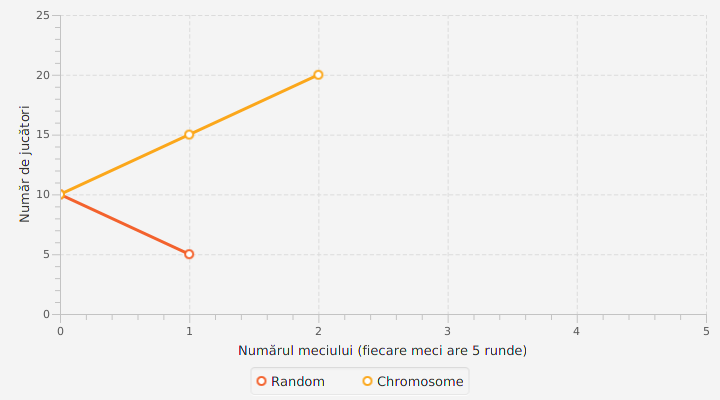
\includegraphics[	
	width=16cm,
	height=7.5cm,
	keepaspectratio
	]{imagini/experiment_4_epoch_1529323027289/chart_from_epoch_1529323309315.png}
	\caption{\textit{Cromozomii câștigă în turneul cu eliminare cu 5 runde/meci.}}
\end{figure}

\begin{figure}[H]
	\centering
	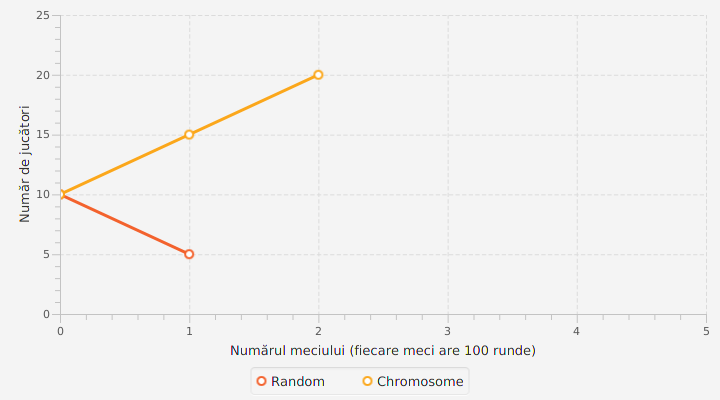
\includegraphics[	
	width=16cm,
	height=7.5cm,
	keepaspectratio
	]{imagini/experiment_4_epoch_1529323027289/chart_from_epoch_1529323321406.png}
	\caption{\textit{Cromozomii câștigă în turneul cu eliminare cu 100 runde/meci.}}
\end{figure}

Strategia din experimentul cu numărul 4 va face față și la un număr de runde mai mic, dar și la un număr de runde mai mare în turneele cu eliminare în fața strategiei \textbf{Random}. Pentru această configurație a turneului eliminatoriu, putem trage concluzia că experimentul numărul 4 oferă o soluție mai bună. 

\subsection{Strategia \textbf{Tit-For-Tat}}

\begin{center}
	\underline{\textit{Experimentul numărul 5}}
\end{center}

\textit{Configurația algoritmului genetic și cea a turneului cu eliminare este trecută în \textbf{Anexa numărul 5}}.\\

Un lucru ce se observă ușor este că strategia \textbf{Tit-For-Tat} reușește să câștige aproape de fiecare dată când la iniţializarea turneului cu eliminare toate strategiile au ponderi egale și numărul de runde/meci este mare.
 
Pentru a bate strategia \textbf{Tit-For-Tat} este necesar un număr mic de runde, fiindcă știm că un meci între doi astfel de indivizi le va crește substanțial scorul, întrucât cooperează la fiecare pas. De asemenea, trebuie să ne folosim de faptul că știm că va coopera la prima mișcare. Strategia inamică se va folosi de faptul că atunci când unul cooperează și celălalt trădează, cel care trădează este mai bine răsplătit decât cel ce a cooperat. În alte cuvinte, strategia inamică trebuie să impersoneze strategia \textbf{Always Defect}.  
 
Cromozomul, cu eleganța reprezentării sale, poate mima toate strategiile standard descrise în capitolele anterioare. Pentru a imita \textbf{Always Defect}, am lăsat ca populația de antrenament să fie dată de un singur individ al acestei strategii, am ales un număr mare de generații (1000), procente mare pentru mutație și încrucișare (50\%), o populație de dimensiuni reduse (15). 
  
\begin{figure}[H]
	\centering
	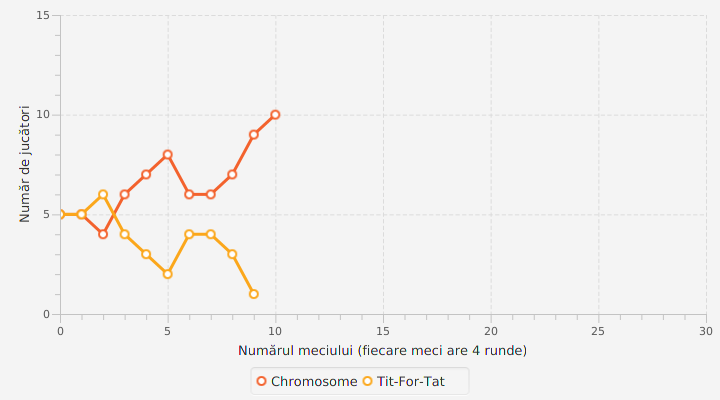
\includegraphics[	
		width=16cm,
		height=7.5cm,
		keepaspectratio
	]{imagini/experiment_5_epoch_1529329866051/chart_from_epoch_1530552284074.png}
	\caption{\textit{Cromozomii câștigă turneul cu eliminare în cadrul unui număr mic de runde, câte 4 runde la fiecare meci al turneului cu eliminare.}}
\end{figure}

Atunci când doi indivizi ce urmează startegia \textbf{Tit-For-Tat} concurează într-un meci, vor coopera la fiecare rundă iar cooperarea mutuală este cea mai bine răsplătită, oferind un punctaj pe măsură. Din acest motiv, la un turneu cu eliminare unde numărul de runde este mai mare (mai mare de 5 runde la fiecare meci), va depăși strategiile care trădează în majoritatea rundelor. 

\begin{figure}[H]
	\centering
	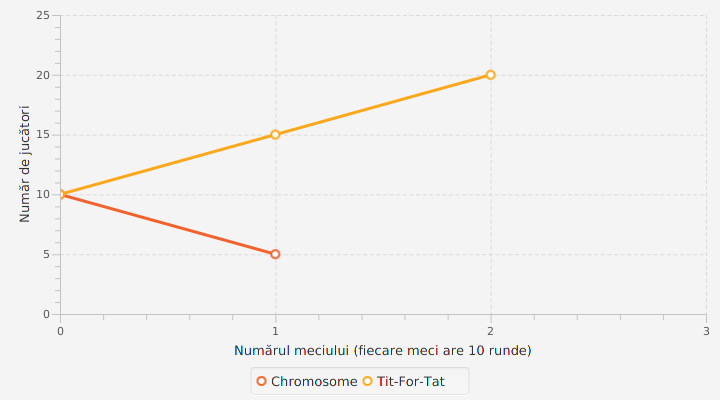
\includegraphics[	
		width=16cm,
		height=7.5cm,
		keepaspectratio
	]{imagini/experiment_5_epoch_1529329866051/chart_from_epoch_1529413879261.png}
	\caption{\textit{Strategia \textbf{Tit-For-Tat} câștigă când numărul de runde este 10.}}
\end{figure}

\begin{center}
	\underline{\textit{Experimentul numărul 6}}
\end{center}

\textit{Configurația algoritmului genetic și cea a turneului cu eliminare este trecută în \textbf{Anexa numărul 6}}.\\

Mai există o altă variantă pentru a învinge o populație dată de copii după \textbf{Tit-For-Tat}. 
 
Am făcut un experiment în care populația de antrenament este dată de un individ cu strategia \textbf{Tit-For-Tat}. Acest lucru a făcut ca strategia oferită de algoritmul genetic să imite strategia \textbf{Tit-For-Tat}. În aceste cazuri, cromozomii și copiile după \textbf{Tit-For-Tat} vor avea același scor și, la rundele eliminatorii, se vor elimina (și apoi duplica) la întâmplare câteva strategii dintre cele două tipuri. Sunt șanse egale de câştig între cele două tipuri de strategii.

\begin{figure}[H]
	\centering
	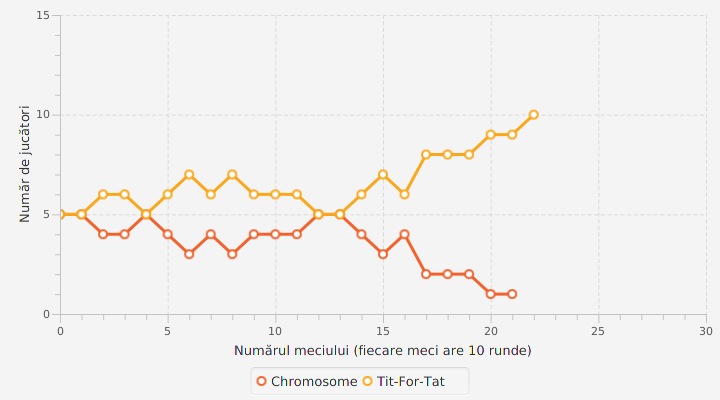
\includegraphics[	
		width=16cm,
		height=7.5cm,
		keepaspectratio
	]{imagini/experiment_6_epoch_1529327580314/chart_from_epoch_1529416356254.png}
	\caption{\textit{Populația ce folosește strategia \textbf{Tit-For-Tat} câștigă.}}
\end{figure}

\begin{figure}[H]
	\centering
	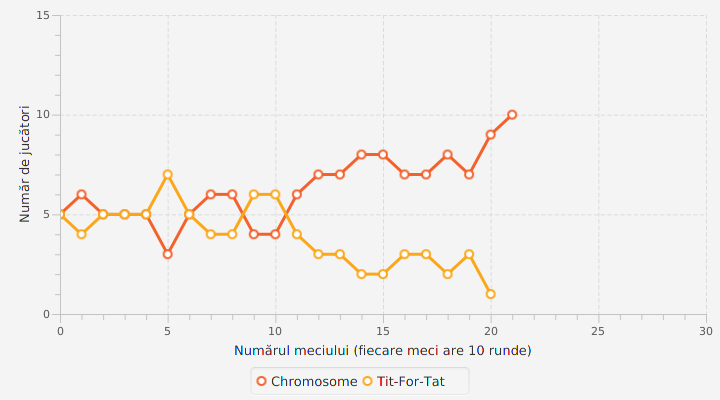
\includegraphics[	
		width=16cm,
		height=7.5cm,
		keepaspectratio
	]{imagini/experiment_6_epoch_1529327580314/chart_from_epoch_1529416343328.png}
	\caption{\textit{Cromozomii câștigă.}}
\end{figure} 











































































































































































































